\documentclass[a4paper]{article}
\usepackage{fancyhdr}
\usepackage{amsmath}
\usepackage{xcolor}
\usepackage{graphicx}
\usepackage{latexsym}
\usepackage{amssymb}

%%clickable links
\usepackage{hyperref}
\hypersetup{
    colorlinks=true, %colore les liens
    breaklinks=true, %permet le retour à la ligne dans les liens trop longs
    urlcolor= blue, %couleur des hyperliens
    linkcolor= black, %couleur des liens internes
}
%formatted algorithm:
\usepackage{algpseudocode}
\usepackage{algorithm}

\algblockdefx[Event]{Event}{EndEvent}%
[1][]{\textbf{Upon event :} #1}%
{}

\algblockdefx[Data]{Data}{EndData}%
[1][]{\textbf{Data :}}%
{}


\algblockdefx[Init]{Init}{EndInit}%
[1][]{\textbf{Initialization :}}%
{}


%% New commands
\newcommand{\eqdef}{\;\stackrel{\text{def}}{=}\;}

\begin{document}
\title{Distributed Systems: Programming Assignment}
\author{David Benamine \& Rodolphe Lepigre\\
        MOSIG - Parallel, Distributed and Embedded Systems}
        \date{\today}
        \maketitle

        %%%%%%%%%%%%%%%%%%%%%%%%%%%%%%%%%%%%%%%%%%%%%%%%%%%%%%%%%%%%%%%%%%%%%%%%%%%%%%
        \section*{Introduction}
        % TODO

        %%%%%%%%%%%%%%%%%%%%%%%%%%%%%%%%%%%%%%%%%%%%%%%%%%%%%%%%%%%%%%%%%%%%%%%%%%%%%%
        \section{Simulator architecture}
        % TODO

        %%%%%%%%%%%%%%%%%%%%%%%%%%%%%%%%%%%%%%%%%%%%%%%%%%%%%%%%%%%%%%%%%%%%%%%%%%%%%%
        \section{Two regular total-order broadcast protocols}
        % TODO

        \subsection{First protocol}
        % TODO (good latency)

        \subsection{Second protocol}
        % TODO (good throughput with N senders)

        %%%%%%%%%%%%%%%%%%%%%%%%%%%%%%%%%%%%%%%%%%%%%%%%%%%%%%%%%%%%%%%%%%%%%%%%%%%%%%
        \section{Theoretical analysis}
        % TODO

        \subsection{First protocol}
        % TODO
        \begin{itemize}
            \item Optimized for latency
            \item Bad throughput
            \item Every broadcast go through the same tree
            \item $P_0$ is always the broadcast initiator
            \item $P_0$ is responsible for the order
            \item if $P_i$ want to send a message, he sent it to 0 who do the broadcast
            \item Latency : log(N) + 1 (send to 0)
            \item Throughput : todo
        \end{itemize}
        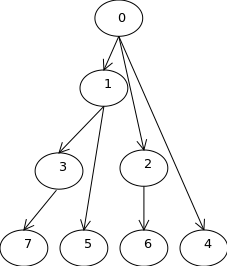
\includegraphics[width=0.5\textwidth]{latencyTO.png}

        \subsubsection{Latency}

        \subsubsection{Throughput}
        % TODO

        \subsection{Second protocol}
        \subsubsection{Principle}
        This protocol is based on the pipeline broadcast protocol but as soon as a node
        receive a message, it will add it to a sorted list. A node $p$ can only deliver the
        first message of its list if this message have been acknowledged by the
        successor of $p$ in the pipeline or if $p$ is the last node of the pipeline.
        This acknowledgement system ensure the total order property (see section
        \ref{sec:pipelineack-proof}).
        \subsubsection{Algorithm}
        \begin{algorithm}[H]
            \centering
            \begin{algorithmic}[5]
                \Data
                \State int : clk
                \Comment{A logical clock}
                \State int : next
                \Comment{the id of the next process in the pipeline}
                \State int : prec
                \Comment{the id of the previous process in the pipeline}
                \State Pending : OrderedList
                \Comment{A list ordered by clock and id}
                \EndData
                \Init
                \State clk$\gets$0
                \State next$\gets$Id()+1\%NProcess
                \If{Id()=0}
                \State prec$\gets$NProcess
                \Else
                \State prec$\gets$Id()-1
                \EndIf
                \State Pending$\gets$EmptyQueue
                \EndInit
                \Event $< tob,Broadcast\ |\ m> $
                \Comment{Start a broadcast}
                \State clk++;
                \State Pending$\rightarrow$add($<m,Id(), clk, false>$) 
                \Comment{The message is added\\}
                \Comment{to the list the false boolean\\}
                \Comment{indicate that we have to wait for one ack}
                \State Send(next,$<m,Id(),clk>$)
                \EndEvent
                \Event $<Receive\ | <m,sender, mclk>>$
                \State clk$\gets$MAX(clk, mclk)+1
                \If{next=sender}
                \State Pending$\rightarrow$add($<m,sender,mclk,true>$)
                \Comment{We are at the end of the pipeline}
                \If{Pending$\rightarrow$IsHead(sender,mclk)}
                \State Pending$\rightarrow$RemoveHead()
                \State Send(prec,$<ack,sender,mclk>$)
                \Comment{m is the first message of\\}
                \Comment{the queue, we can acknowledge it}
                \State Deliver(sender,m)
                \Comment{And deliver it}
                \EndIf
                \Else
                \State Pending$\rightarrow$add($<m,sender,mclk,false>$)
                \State Send(next,$<m,sender,mclk>$)
                \Comment{We forward m through the pipeline}
                \EndIf
                \EndEvent
                \algstore{myalg}
            \end{algorithmic}
            \caption{Pipeline based total ordered broadcast protocol}
        \end{algorithm}
        \begin{algorithm}[H]
            \centering
            \begin{algorithmic}[5]
                \algrestore{myalg}

                \Event $<Receive\  | <ack,sender, mclk>>$
                \State clk$\gets$ Max(clk,mlck)+1
                \If{Pending$\rightarrow$IsHead(sender,mclk)}
                \Comment{m is the head\\}
                \Comment{we can deliver it}
                \State m$gets$(Pending$\rightarrow$RemoveHead())
                \State Deliver(sender,m)
                \If{sender$\neq$ Id()}
                \Comment{We have to forward the ack}
                \State Send(prec,$<ack,sender,mclk>$
                \EndIf
                \State $<m,sender,mclk,b>\gets$Pending$\rightarrow$getHead()
                \While{b}
                \Comment{While we have receive an ack for\\}
                \Comment{the message at the head of the queue\\}
                \Comment{we can deliver it and forward the ack}
                \State Pending$\rightarrow$RemoveHead()
                \State Deliver(sender,m)
                \If{sender$\neq$ Id()}
                \Comment{We have to forward the ack}
                \State Send(prec,$<ack,sender,mclk>$
                \EndIf
                \State $<m,sender,mclk,b>\gets$(Pending$\rightarrow$getHead())
                \EndWhile
                \Else
                \Comment{m isn't the head we mark m as acknowledged\\}
                \Comment{but we won't forward the ack and deliver it\\}
                \Comment{until m is the head of the pending queue}
                \State Pending$\rightarrow$Remove($<m,sender,mclk,false>$)
                \State Pending$\rightarrow$Add($<m,sender,mclk,true>$)
                \EndIf
                \EndEvent
            \end{algorithmic}
        \end{algorithm}
        \subsubsection{Proof}
        \begin{itemize}
            \item Validity : As there  is no crashes, if a process P broadcast a
                message m, m will be received by every process. If the last
                process haven't any message in it's queue, he will acknowledge
                and deliver m. 
        \end{itemize}
        \label{sec:pipelineack-proof}
        \subsubsection{Latency}
        % TODO

        \subsubsection{Throughput}
        % TODO

        %%%%%%%%%%%%%%%%%%%%%%%%%%%%%%%%%%%%%%%%%%%%%%%%%%%%%%%%%%%%%%%%%%%%%%%%%%%%%%
        \section{Empirical evaluation}
        % TODO

        %%%%%%%%%%%%%%%%%%%%%%%%%%%%%%%%%%%%%%%%%%%%%%%%%%%%%%%%%%%%%%%%%%%%%%%%%%%%%%
        \section*{Conclusion}
        % TODO

        \end{document}

